% -----------------------------------------------------------------------------
% Material de apoio: não integra os 18 min 15 s da narrativa principal.
% -----------------------------------------------------------------------------

\backupbegin

\section{Complemento: boas práticas de Ciência de Dados}

% Complemento 1 ---------------------------------------------------------------
\begin{frame}{Desafios na seleção dos datasets}
  \begin{beamercolorbox}[wd=\linewidth,sep=.12cm,rounded=true]{block title}
    \centering\sffamily\bfseries\fontsize{10.5}{12.6}\selectfont
    Disponibilidade pública não implica adequação ao desenho experimental
  \end{beamercolorbox}

  \vspace{.12cm}
  \begin{columns}[T,onlytextwidth]
    \begin{column}{0.31\textwidth}
      \begin{beamercolorbox}[wd=\linewidth,sep=.16cm,rounded=true]{block body}
        {\sffamily\bfseries\color{CoInfoBlue}1. Busca e avaliação}\par\vspace{.08cm}
        {\fontsize{8.5}{10.2}\selectfont
          Alvo defensável, canais interpretáveis, volume para Monte Carlo e documentação suficiente.}
      \end{beamercolorbox}
    \end{column}
    \begin{column}{0.34\textwidth}
      \begin{beamercolorbox}[wd=\linewidth,sep=.16cm,rounded=true]{takeaway}
        {\sffamily\bfseries\color{CoInfoRose}2. Dois candidatos adiados}\par\vspace{.08cm}
        {\fontsize{8.5}{10.2}\selectfont
          CSI Wi-Fi e sistema hidráulico: sessões, janelas e ciclos com dependência temporal exigiriam outra unidade amostral e validação própria.}
      \end{beamercolorbox}
    \end{column}
    \begin{column}{0.31\textwidth}
      \begin{beamercolorbox}[wd=\linewidth,sep=.16cm,rounded=true]{block body}
        {\sffamily\bfseries\color{CoInfoMint}3. Três cenários selecionados}\par\vspace{.08cm}
        {\fontsize{8.5}{10.2}\selectfont
          Occupancy, Air Quality e SUPPORT2: estrutura tabular; preparação, alvo e preditores definidos por cenário.}
      \end{beamercolorbox}
    \end{column}
  \end{columns}

  \vspace{.12cm}
  \begin{beamercolorbox}[wd=\linewidth,sep=.12cm,rounded=true]{takeaway}
    \centering\sffamily\bfseries\fontsize{10.1}{12.0}\selectfont
    O desafio foi compatibilizar domínio, unidade amostral e método de avaliação.
  \end{beamercolorbox}
  \sourcecite{Relatório final, capítulo 4 e seção 10.6.}

  \speakernotes
    {A busca começou com várias bases públicas, mas disponibilidade não era o critério decisivo. O protocolo precisava de um alvo defensável, canais interpretáveis, volume para as simulações de Monte Carlo e documentação que permitisse reconstruir a preparação. Dois candidatos foram adiados: dados CSI de Wi-Fi e monitoramento de um sistema hidráulico. Neles, sessões, janelas e ciclos introduzem dependência temporal. Incorporá-los corretamente exigiria definir outra unidade amostral, agrupar observações correlacionadas e adotar validação temporal ou por sessão. Isso desviaria o trabalho do objetivo central, que é comparar a estrutura de cooperação entre subconjuntos em uma representação tabular. Por isso foram selecionados Occupancy, Air Quality e SUPPORT2, cada um ainda com decisões próprias de alvo, partição e preditores.}
    {Depois da seleção, o próximo passo é controlar e registrar o caminho percorrido pelos dados em cada cenário.}
    {A seleção foi orientada pela compatibilidade entre o dataset e o protocolo, não apenas pela disponibilidade pública.}
    {Entre 45 e 60 segundos; slide opcional, fora da duração principal.}
    {Não dizer que séries temporais são inadequadas; dizer que exigiriam modelagem e validação fora do escopo atual.}
\end{frame}

% Complemento 2 ---------------------------------------------------------------
\begin{frame}{Proveniência e integridade experimental}
  \begin{beamercolorbox}[wd=\linewidth,sep=.12cm,rounded=true]{block title}
    \centering\sffamily\bfseries\fontsize{10.7}{12.8}\selectfont
    Proveniência = origem + transformação + partição + uso
  \end{beamercolorbox}

  \vspace{.10cm}
  \begin{columns}[T,onlytextwidth]
    \begin{column}{0.24\textwidth}
      \begin{beamercolorbox}[wd=\linewidth,sep=.12cm,rounded=true]{block body}
        {\sffamily\bfseries\fontsize{9.0}{10.7}\selectfont\color{CoInfoBlue}Origem documentada}\par\vspace{.04cm}
        {\fontsize{8.0}{9.5}\selectfont Fonte, DOI, arquivo canônico e hash SHA-256 registrados.}
      \end{beamercolorbox}
    \end{column}
    \begin{column}{0.24\textwidth}
      \begin{beamercolorbox}[wd=\linewidth,sep=.12cm,rounded=true]{block body}
        {\sffamily\bfseries\fontsize{9.0}{10.7}\selectfont\color{CoInfoBlue}Papéis explícitos}\par\vspace{.04cm}
        {\fontsize{8.0}{9.5}\selectfont Reservatório de treinamento separado do teste real fixo.}
      \end{beamercolorbox}
    \end{column}
    \begin{column}{0.24\textwidth}
      \begin{beamercolorbox}[wd=\linewidth,sep=.12cm,rounded=true]{block body}
        {\sffamily\bfseries\fontsize{9.0}{10.7}\selectfont\color{CoInfoBlue}Transformações}\par\vspace{.04cm}
        {\fontsize{8.0}{9.5}\selectfont Alvo, coorte, partição e padronização descritos.}
      \end{beamercolorbox}
    \end{column}
    \begin{column}{0.24\textwidth}
      \begin{beamercolorbox}[wd=\linewidth,sep=.12cm,rounded=true]{block body}
        {\sffamily\bfseries\fontsize{9.0}{10.7}\selectfont\color{CoInfoBlue}Uso controlado}\par\vspace{.04cm}
        {\fontsize{8.0}{9.5}\selectfont Geradores e pré-processamento parametrizados apenas no treino.}
      \end{beamercolorbox}
    \end{column}
  \end{columns}

  \vspace{.09cm}
  {\centering\sffamily\fontsize{8.5}{10.2}\selectfont\color{CoInfoGray}
    O teste real informa a avaliação, mas não a parametrização dos geradores nem as decisões de preparação.\par}

  \vspace{.08cm}
  \begin{beamercolorbox}[wd=\linewidth,sep=.12cm,rounded=true]{takeaway}
    \centering\sffamily\bfseries\fontsize{10.2}{12.1}\selectfont
    O resultado só é interpretável porque o caminho dos dados foi controlado.
  \end{beamercolorbox}
  \sourcecite{Relatório final, capítulos 4 e 5; catálogos e relatórios de datasets do CoInfoSim.}

  \speakernotes
    {Em Ciência de Dados, proveniência não significa apenas saber de qual site veio um arquivo. Ela descreve toda a trajetória: qual arquivo canônico foi usado, como sua integridade foi verificada, como o alvo e a coorte foram definidos, como as linhas foram particionadas e em que etapa cada transformação foi estimada. No CoInfoSim, os papéis de reservatório de treinamento e teste real fixo são explícitos. Padronização e parametrização dos modelos geradores usam somente o treinamento; o teste fica reservado para avaliação comum dos três braços. Os hashes dos arquivos e as impressões digitais das partições ajudam a detectar trocas silenciosas de dados.}
    {Se houver interesse na infraestrutura que torna esse controle auditável, o próximo slide mostra o que foi persistido.}
    {Proveniência é a história completa do dado dentro do experimento, não apenas sua origem externa.}
    {Cerca de 1 minuto; slide opcional, fora da duração principal.}
    {Não afirmar ausência absoluta de qualquer risco de vazamento; afirmar os controles concretos implementados e documentados.}
\end{frame}

% Complemento 3 ---------------------------------------------------------------
\begin{frame}{Reprodutibilidade computacional}
  \begin{columns}[T,onlytextwidth]
    \begin{column}{0.54\textwidth}
      \begin{beamercolorbox}[wd=\linewidth,sep=.13cm,rounded=true]{block body}
        {\sffamily\bfseries\color{CoInfoBlue}Cada execução registra}\par\vspace{.04cm}
        \begin{itemize}\fontsize{8.4}{10.0}\selectfont\setlength{\itemsep}{.02cm}
          \item sementes, grade de $n$, braços, classificadores e subconjuntos;
          \item padronização, alvo, parâmetros da Gaussiana e componentes do GMM;
          \item hashes dos arquivos e impressões digitais das partições;
          \item replicações, parada, execução computacional, versão e IDs.
          \item resultados que regeneram relatórios e figuras sem repetir o Monte Carlo.
        \end{itemize}
      \end{beamercolorbox}
    \end{column}
    \begin{column}{0.43\textwidth}
      \begin{beamercolorbox}[wd=\linewidth,sep=.12cm,rounded=true]{block body}
        {\sffamily\bfseries\color{CoInfoBlue}Reprodutibilidade}\par
        {\fontsize{8.2}{9.8}\selectfont Executar novamente o mesmo protocolo com os mesmos artefatos e configuração.}
      \end{beamercolorbox}

      \vspace{.09cm}
      \begin{beamercolorbox}[wd=\linewidth,sep=.12cm,rounded=true]{block body}
        {\sffamily\bfseries\color{CoInfoPlum}Replicabilidade}\par
        {\fontsize{8.2}{9.8}\selectfont Obter evidência compatível em novas execuções, implementações ou cenários.}
      \end{beamercolorbox}

    \end{column}
  \end{columns}

  \vspace{.09cm}
  \begin{beamercolorbox}[wd=\linewidth,sep=.12cm,rounded=true]{takeaway}
    \centering\sffamily\bfseries\fontsize{10.2}{12.1}\selectfont
    Não basta rodar o experimento: é preciso poder auditar como ele foi rodado.
  \end{beamercolorbox}
  \sourcecite{Relatório final, seção 5.8; README e artefatos persistidos em \texttt{output/reports}.}

  \speakernotes
    {Este ponto importa em uma disciplina de Ciência de Dados porque um número sem contexto de execução é difícil de auditar. O CoInfoSim persiste a configuração científica, a configuração computacional e os resultados necessários para reconstruir a análise: sementes, grade amostral, classificadores, subconjuntos, parâmetros dos geradores, hashes, partições, contagens de replicação, critérios de parada, versão e identificadores. A hierarquia de relatórios pode ser regenerada a partir desses artefatos sem repetir o Monte Carlo. Uso aqui uma distinção conservadora: isso sustenta reprodutibilidade computacional do protocolo; replicabilidade exigiria evidência compatível em novas execuções, implementações ou contextos independentes.}
    {A infraestrutura reprodutível também foi empacotada para uso fora deste checkout de pesquisa.}
    {Auditoria exige preservar tanto o resultado quanto as condições que o produziram.}
    {Cerca de 1 minuto; slide opcional, fora da duração principal.}
    {Não reivindicar replicação independente completa nem equivalência garantida em ambientes e versões arbitrários.}
\end{frame}

% Complemento 4 ---------------------------------------------------------------
\begin{frame}{Software científico aberto}
  \begin{columns}[T,onlytextwidth]
    \begin{column}{0.43\textwidth}
      \begin{beamercolorbox}[wd=\linewidth,sep=.16cm,rounded=true]{block title}
        {\color{white}\ttfamily\fontsize{8.4}{10.4}\selectfont
          python -m pip install coinfosim\par\medskip
          coinfosim --help\par\medskip
          coinfosim scenario run occupancy\par
          \hspace{1.2em}--mode smoke}
      \end{beamercolorbox}

      \vspace{.10cm}
      \begin{beamercolorbox}[wd=\linewidth,sep=.14cm,rounded=true]{takeaway}
        {\sffamily\fontsize{8.5}{10.2}\selectfont
          Software: GPL-3.0-or-later.\par
          Datasets: licenças e requisitos de atribuição tratados separadamente.}
      \end{beamercolorbox}
    \end{column}
    \begin{column}{0.54\textwidth}
      \begin{beamercolorbox}[wd=\linewidth,sep=.16cm,rounded=true]{block body}
        \begin{itemize}\fontsize{9.0}{10.8}\selectfont\setlength{\itemsep}{.10cm}
          \item código, documentação e histórico versionados no GitHub;
          \item pacote \texttt{coinfosim} publicado no PyPI;
          \item CLI para cenários, datasets, execuções, configuração e publicação;
          \item relatórios HTML, figuras e resultados persistidos produzidos pelo fluxo;
          \item regeneração de relatórios e inspeção de execuções pela própria CLI.
        \end{itemize}
      \end{beamercolorbox}
    \end{column}
  \end{columns}

  \vspace{.09cm}
  \begin{beamercolorbox}[wd=\linewidth,sep=.12cm,rounded=true]{takeaway}
    \centering\sffamily\bfseries\fontsize{10.2}{12.1}\selectfont
    O projeto foi organizado como infraestrutura científica reutilizável.
  \end{beamercolorbox}
  \sourcecite{README e \texttt{pyproject.toml}; GitHub \texttt{paulorenatoaz/coinfosim}; PyPI \texttt{coinfosim} 0.2.1, verificado em 16 jul. 2026.}

  \speakernotes
    {A prática de Ciência de Dados não termina quando um notebook produz uma figura. O CoInfoSim foi organizado como pacote Python instalável, com código e documentação versionados no GitHub e uma interface de linha de comando. A publicação do pacote coinfosim no PyPI foi verificada; a instalação documentada é feita com pip. Pela CLI, o usuário pode listar e executar cenários, verificar datasets, inspecionar registros de execução e regenerar relatórios. Os fluxos produzem relatórios HTML, figuras e resultados persistidos. A licença GPL cobre o software, enquanto cada dataset mantém seus próprios termos de uso e atribuição. Essa separação é parte da responsabilidade de publicar software científico.}
    {O último complemento aplica essa responsabilidade ao caso mais sensível do estudo, o SUPPORT2.}
    {Reutilização científica depende de empacotamento, documentação e interfaces verificáveis.}
    {Cerca de 1 minuto; slide opcional, fora da duração principal.}
    {Não prometer estabilidade permanente da API, revisão formal de contribuições ou garantias de CI além do que está documentado.}
\end{frame}

% Complemento 5 ---------------------------------------------------------------
\begin{frame}{SUPPORT2 — uso responsável no experimento}
  \begin{beamercolorbox}[wd=\linewidth,sep=.17cm,rounded=true]{block body}
    {\sffamily\bfseries\color{CoInfoBlue}Boas práticas metodológicas}\par\vspace{.07cm}
    \begin{itemize}\fontsize{9.0}{10.8}\selectfont\setlength{\itemsep}{.07cm}
      \item base pública de pesquisa, com origem e versão documentadas;
      \item identificador utilizado somente na preparação e auditoria das partições, sendo removido antes do treinamento;
      \item variáveis de construção do alvo, \texttt{death} e \texttt{d.time}, excluídas dos preditores;
      \item desfechos alternativos e proxies, \texttt{hospdead}, \texttt{surv2m} e \texttt{surv6m}, também excluídos;
      \item análise metodológica e agregada, sem finalidade diagnóstica ou recomendação clínica.
    \end{itemize}
  \end{beamercolorbox}

  \vspace{.12cm}
  \begin{beamercolorbox}[wd=\linewidth,sep=.12cm,rounded=true]{takeaway}
    \centering\sffamily\bfseries\fontsize{10.0}{11.9}\selectfont
    Dados médicos públicos continuam exigindo proveniência, controle de vazamento e limites claros de interpretação.
  \end{beamercolorbox}
  \sourcecite{SUPPORT2: DOI 10.3886/ICPSR02957.v2; HBiostat; protocolo descrito no capítulo 4 do relatório final.}

  \speakernotes
    {No SUPPORT2, responsabilidade é apresentada por meio de decisões metodológicas verificáveis. A origem e a versão da base estão documentadas. O identificador sequencial participa apenas da preparação e da auditoria das partições e é removido antes do treinamento. As variáveis \texttt{death} e \texttt{d.time} são usadas para construir o alvo de mortalidade em 180 dias e, por isso, não entram como preditores. Também são excluídos o desfecho hospitalar e as estimativas de sobrevivência \texttt{hospdead}, \texttt{surv2m} e \texttt{surv6m}, que poderiam antecipar diretamente o resultado. O objetivo é metodológico e agregado: avaliar preservação estrutural, não produzir diagnóstico individual ou recomendação clínica.}
    {A partir daqui, os demais slides de apoio retomam fórmulas, configurações e tabelas detalhadas do experimento.}
    {Responsabilidade aparece em proveniência, prevenção de vazamento e limites de interpretação.}
    {Entre 45 e 60 segundos; slide opcional, fora da duração principal.}
    {Não apresentar o cenário como validação clínica nem fazer afirmações adicionais sobre identificação ou licenciamento que não sejam necessárias ao método.}
\end{frame}

% Apoio 1 ---------------------------------------------------------------------
\begin{frame}{Definições formais das três métricas}
  \begin{columns}[T,onlytextwidth]
    \begin{column}{0.49\textwidth}
      \begin{beamercolorbox}[wd=\linewidth,sep=.11cm,rounded=true]{block body}
        {\bfseries\color{CoInfoBlue}Correlação de ranking}\par
        {\fontsize{8.5}{10.1}\selectfont Postos por perda média nos dois braços:}\par\vspace{.05cm}
        \resizebox{0.86\linewidth}{!}{$
          \rho_{\mathrm{rank}}^{(g,f)}(n)=
          \operatorname{corr}_{\mathrm{Spearman}}
          \!\left(\mathbf r^{(R,f)}(n),\mathbf r^{(g,f)}(n)\right).$}
      \end{beamercolorbox}
    \end{column}
    \begin{column}{0.49\textwidth}
      \begin{beamercolorbox}[wd=\linewidth,sep=.11cm,rounded=true]{block body}
        {\bfseries\color{CoInfoBlue}\WA}\par
        {\fontsize{8.5}{10.1}\selectfont $\mathcal P_{\mathrm{valid}}$: pares sem empate em ambos os braços.}\par\vspace{.05cm}
        \resizebox{0.88\linewidth}{!}{$
          \mathrm{WA}^{(g,f)}(n)=
          \frac{\sum_{(i,j)\in\mathcal P_{\mathrm{valid}}}
          \mathbf 1\!\left\{W^{(R,f)}_{ij}=W^{(g,f)}_{ij}\right\}}
          {|\mathcal P_{\mathrm{valid}}|}.$}
      \end{beamercolorbox}
    \end{column}
  \end{columns}

  \vspace{.10cm}
  \begin{beamercolorbox}[wd=\linewidth,sep=.11cm,rounded=true]{block body}
    {\bfseries\color{CoInfoBlue}Último cruzamento dirigido e similaridade progressiva}\par\vspace{.05cm}
    \begin{columns}[T,onlytextwidth]
      \begin{column}{0.48\textwidth}
        \resizebox{0.90\linewidth}{!}{$
          N_{ij}^{\star}(n_t)=\max\!\left\{n_k\le n_t:
          \Delta_{ij}(n_{k-1})\ge0,\ \Delta_{ij}(n_k)<0\right\}.$}
        \vspace{.06cm}

        {\fontsize{8.2}{9.7}\selectfont O evento é dirigido e atribuído ao ponto observado da grade, sem interpolação; registra-se o último evento do prefixo.}
      \end{column}
      \begin{column}{0.49\textwidth}
        \resizebox{0.90\linewidth}{!}{$
          J(t)=\frac{|C_R(t)\cap C_g(t)|}{|C_R(t)\cup C_g(t)|},\qquad
          d(t)=\underset{C_R\cap C_g}{\operatorname{média}}
          |\log_2N^{\star,g}_{ij}-\log_2N^{\star,R}_{ij}|.$}
        \vspace{.08cm}

        \resizebox{0.88\linewidth}{!}{$
          T(t)=\operatorname{clip}_{[0,1]}\!\left(1-
          \frac{d(t)}{\log_2 n_t-\log_2 n_1}\right),\qquad
          \mathrm{NS}(t)=J(t)\,T(t).$}
        \vspace{.05cm}

        {\fontsize{8.2}{9.7}\selectfont $C_R,C_g$: células dirigidas com cruzamento definido.}
      \end{column}
    \end{columns}
  \end{beamercolorbox}

  \vspace{.08cm}
  {\fontsize{7.8}{9.4}\selectfont\color{CoInfoGray}
    $R$: braço real; $g$: braço sintético; $f$: classificador; $\Delta_{ij}$: diferença das perdas médias do par dirigido.}
  \sourcecite{capítulo 6 do relatório final; Spearman (1904).}
\end{frame}

% Apoio 2 ---------------------------------------------------------------------
\begin{frame}{Datasets, partições e espaço de subconjuntos}
  \centering
  \renewcommand{\arraystretch}{1.20}
  \fontsize{8.3}{10}\selectfont
  \begin{tabularx}{\linewidth}{>{\bfseries}p{1.60cm}cc>{\raggedright\arraybackslash}p{2.30cm}>{\raggedright\arraybackslash}p{2.30cm}>{\raggedright\arraybackslash}X}
    \toprule
    Dataset & Canais & Subconj. & Reservatório de treino & Teste real fixo & Partição e alvo \\
    \midrule
    Occupancy & 5 & 31 & 8.143 (6.414/1.729) & 12.417 (9.396/3.021) & Partição original; ocupação binária; sem imputação. \\
    Air Quality & 5 & 31 & 7.192 (5.374/1.818) & 1.799 (1.524/275) & Corte cronológico 80/20; $C6H6(GT)\ge14{,}5$, percentil 75 calculado apenas no treino. \\
    SUPPORT2 & 7 & 127 & 7.098 (3.768/3.330) & 1.775 (943/832) & 80/20, semente 0, estratificação conjunta; óbito até 180 dias. \\
    \bottomrule
  \end{tabularx}

  \vspace{0.19cm}
  \begin{columns}[T,onlytextwidth]
    \begin{column}{0.31\textwidth}
      \resultcard{CoInfoBlue}{Occupancy}
        {$X_1$ temperatura; $X_2$ umidade; $X_3$ luz}
        {$X_4$ CO$_2$; $X_5$ razão de umidade}
    \end{column}
    \begin{column}{0.31\textwidth}
      \resultcard{CoInfoAmber}{Air Quality}
        {cinco respostas de sensores PT08}
        {alvo derivado da referência de benzeno}
    \end{column}
    \begin{column}{0.34\textwidth}
      \resultcard{CoInfoMint}{SUPPORT2}
        {pressão, frequência cardíaca/respiratória, temperatura}
        {leucócitos, creatinina e sódio}
    \end{column}
  \end{columns}
  \sourcecite{Candanedo e Feldheim (2016); De Vito et al. (2008); SUPPORT Principal Investigators (1995); Knaus et al. (1995).}
\end{frame}

% Apoio 3 ---------------------------------------------------------------------
\begin{frame}{Configurações dos geradores e classificadores}
  \fontsize{9.65}{11.35}\selectfont
  \begin{columns}[T,onlytextwidth]
    \begin{column}{0.49\textwidth}
      \eyebrow{Modelos geradores por classe}
      \vspace{0.12cm}
      \begin{beamercolorbox}[wd=\linewidth,sep=.14cm,rounded=true]{block body}
        {\bfseries Gaussiana única}\par
        parametrizada a partir dos dados reais de treinamento: média e covariância amostrais no espaço padronizado completo;
        \texttt{ddof=1}; ridge diagonal apenas se necessário ($10^{-10}$ a $10^{-3}$).
      \end{beamercolorbox}
      \vspace{0.12cm}
      \begin{beamercolorbox}[wd=\linewidth,sep=.14cm,rounded=true]{block body}
        {\bfseries GMM}\par
        parametrizado a partir dos mesmos dados reais; covariância completa; $K=1,\ldots,5$; mínimo de 50 observações por componente; menor BIC por classe; \texttt{reg\_covar=$10^{-6}$}, \texttt{n\_init=5}.\par
        {\fontsize{8.3}{9.8}\selectfont $K$ escolhido: Occupancy 5/5; Air Quality 5/4; SUPPORT2 5/5.}
      \end{beamercolorbox}
    \end{column}
    \begin{column}{0.48\textwidth}
      \eyebrow{Classificadores}
      \vspace{0.12cm}
      \begin{beamercolorbox}[wd=\linewidth,sep=.14cm,rounded=true]{block body}
        \fontsize{9.7}{11.5}\selectfont
        \begin{itemize}\setlength{\itemsep}{.04cm}
          \item SVM linear: \texttt{SVC(kernel="linear")};
          \item Regressão Logística: \texttt{max\_iter=1000};
          \item Gaussian Naive Bayes: padrões da versão executada;
          \item Random Forest no SUPPORT2: 100 árvores, profundidade 12, folha mínima 5, \texttt{max\_features="sqrt"}.
        \end{itemize}
      \end{beamercolorbox}
      \vspace{0.10cm}
      {\fontsize{8.7}{10.4}\selectfont
        A configuração do Random Forest foi calibrada somente no reservatório real e congelada antes dos três braços.}
    \end{column}
  \end{columns}
  \sourcecite{McLachlan e Peel (2000); Schwarz (1978); Cortes e Vapnik (1995); Hosmer et al. (2013); Hand e Yu (2001); Breiman (2001); Pedregosa et al. (2011).}
\end{frame}

% Apoio 4 ---------------------------------------------------------------------
\begin{frame}{Resultados adicionais — Occupancy e Air Quality}
  \eyebrow{Métricas estruturais em $n=512$}
  \vspace{0.06cm}
  \centering
  \renewcommand{\arraystretch}{1.0}
  \fontsize{7.4}{8.9}\selectfont
  \begin{tabular}{llccc}
    \toprule
    Dataset / classificador & Treinamento $\rightarrow$ teste & $\rankrho$ & \WA{} & Sim. de \Nstar{} \\
    \midrule
    \multirow{6}{*}{\shortstack[l]{Occupancy}}
      & SVM, Gaussiana única $\rightarrow$ Real & 0,9528 & 0,9204 & 0,4479 \\
      & SVM, GMM $\rightarrow$ Real & 0,8774 & 0,8624 & 0,4949 \\
      & Reg. Logística, Gaussiana única $\rightarrow$ Real & 0,9036 & 0,8839 & 0,5302 \\
      & Reg. Logística, GMM $\rightarrow$ Real & 0,8738 & 0,8903 & 0,6243 \\
      & Gaussian NB, Gaussiana única $\rightarrow$ Real & 0,9976 & 0,9892 & 0,2452 \\
      & Gaussian NB, GMM $\rightarrow$ Real & 0,9996 & 0,9978 & 0,5490 \\
    \midrule
    \multirow{6}{*}{\shortstack[l]{Air Quality}}
      & SVM, Gaussiana única $\rightarrow$ Real & 0,8944 & 0,8882 & 0,2087 \\
      & SVM, GMM $\rightarrow$ Real & 0,9580 & 0,9333 & 0,2965 \\
      & Reg. Logística, Gaussiana única $\rightarrow$ Real & 0,9359 & 0,9118 & 0,4646 \\
      & Reg. Logística, GMM $\rightarrow$ Real & 0,9839 & 0,9613 & 0,6102 \\
      & Gaussian NB, Gaussiana única $\rightarrow$ Real & 1,0000 & 1,0000 & 0,7294 \\
      & Gaussian NB, GMM $\rightarrow$ Real & 0,9996 & 0,9978 & 0,8085 \\
    \bottomrule
  \end{tabular}

  \vspace{0.08cm}
  {\fontsize{7.9}{9.4}\selectfont\color{CoInfoGray}
    Para \Nstar{}, o valor em 512 resume os últimos cruzamentos dirigidos no prefixo $2,\ldots,512$. No full-scale 000006 (grade até 1.024), os valores do Gaussian NB em $n=512$ coincidem; em $n=1024$: 1,0000 / 1,0000 / 0,7319 (Gaussiana única) e 1,0000 / 1,0000 / 0,8095 (GMM).}
  \sourcecite{relatórios dos cenários Occupancy 000002, Air Quality 000005 e 000006; tabelas do capítulo 7 do relatório final.}
\end{frame}

% Apoio 5 ---------------------------------------------------------------------
\begin{frame}{Curvas cooperativas do Air Quality (Gaussian NB)}
  \centering
  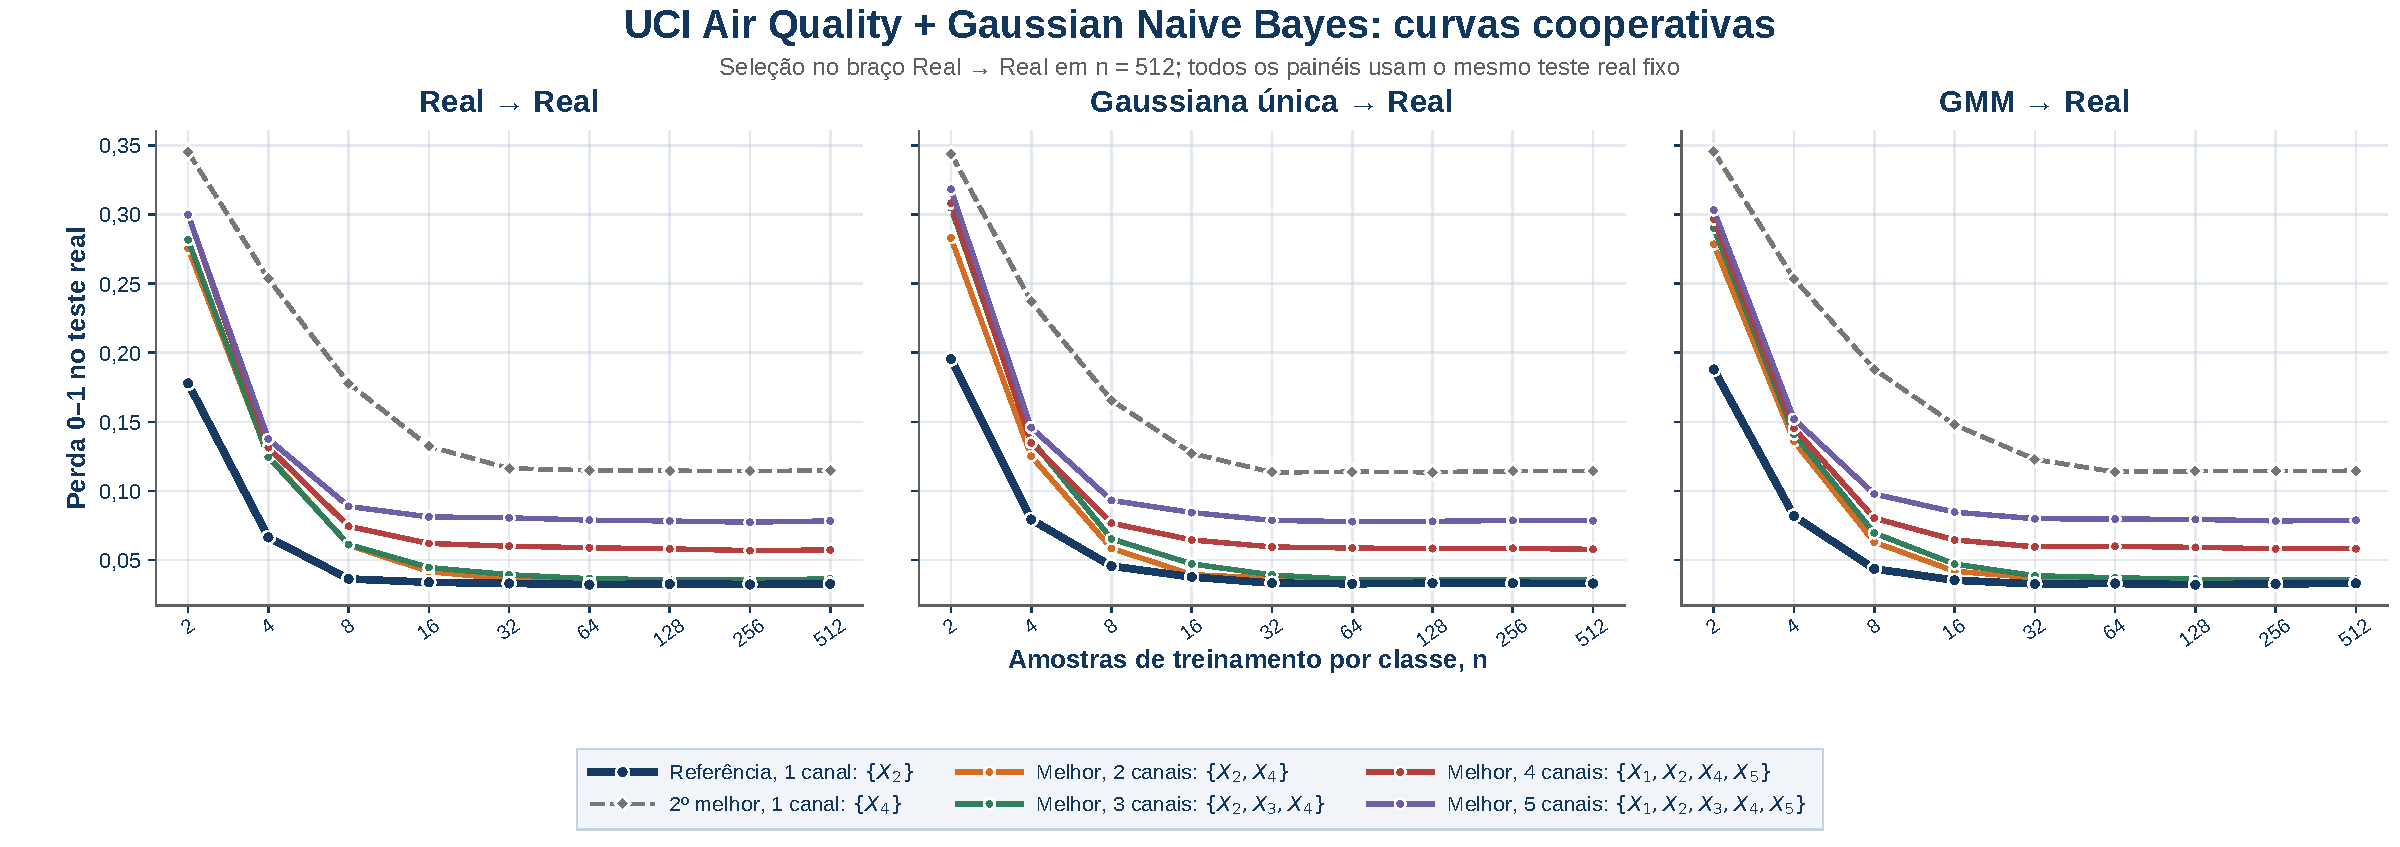
\includegraphics[width=0.94\linewidth,height=4.90cm,keepaspectratio]{figures/air_quality_gnb_curvas_pt.pdf}

  \vspace{0.08cm}
  {\fontsize{8.2}{9.8}\selectfont\color{CoInfoGray}
    A organização das curvas é muito semelhante nos três braços: $\{X_2\}$ domina desde amostras pequenas — a base dos valores quase perfeitos de ranking e \WA{} do slide 10.}
  \sourcecite{perdas persistidas das simulações 000015--000017, vinculadas ao cenário Air Quality full 000005.}
\end{frame}

% Apoio 6 ---------------------------------------------------------------------
\begin{frame}{Resultados adicionais — SUPPORT2}
  \begin{columns}[T,onlytextwidth]
    \begin{column}{0.61\textwidth}
      \centering
      \renewcommand{\arraystretch}{1.07}
      \fontsize{6.9}{8.3}\selectfont
      \begin{tabular}{lccc}
        \toprule
        Classificador, treinamento $\rightarrow$ teste & $\rankrho$ & WA & Sim. \Nstar{} \\
        \midrule
        SVM, Gaussiana única $\rightarrow$ Real & 0,8672 & 0,8614 & 0,3076 \\
        SVM, GMM $\rightarrow$ Real & 0,9708 & 0,9344 & 0,4145 \\
        Reg. Log., Gaussiana única $\rightarrow$ Real & 0,9853 & 0,9514 & 0,2932 \\
        Reg. Log., GMM $\rightarrow$ Real & 0,9827 & 0,9461 & 0,3169 \\
        Gaussian NB, Gaussiana única $\rightarrow$ Real & 0,7915 & 0,7951 & 0,3196 \\
        Gaussian NB, GMM $\rightarrow$ Real & 0,9144 & 0,8715 & 0,4590 \\
        \midrule
        Random Forest, Gaussiana única $\rightarrow$ Real & 0,8387 & 0,8282 & 0,6799 \\
        Random Forest, GMM $\rightarrow$ Real & 0,8665 & 0,8429 & 0,6340 \\
        \bottomrule
      \end{tabular}
    \end{column}
    \begin{column}{0.36\textwidth}
      \eyebrow{Random Forest: \Nstar{} denso}
      \vspace{0.12cm}
      \begin{beamercolorbox}[wd=\linewidth,sep=.14cm,rounded=true]{block body}
        \fontsize{8.5}{10.2}\selectfont
        \textbf{Referência real:} 11.948 cruzamentos definidos.\par
        \vspace{.09cm}
        \textbf{Gaussiana única:} 11.637 definidos; 10.521 compartilhados; Jaccard 0,8053; temporal 0,8442.\par
        \vspace{.09cm}
        \textbf{GMM:} 11.531 definidos; 10.200 compartilhados; Jaccard 0,7681; temporal 0,8254.\par
      \end{beamercolorbox}
      \vspace{.14cm}
      {\fontsize{8.2}{9.8}\selectfont\color{CoInfoGray}
        A concordância não resulta de matrizes quase vazias.\par}
    \end{column}
  \end{columns}
  \sourcecite{cenários SUPPORT2 000007 e 000008; tabelas do capítulo 7 do relatório final.}
\end{frame}

% Apoio 7 ---------------------------------------------------------------------
\begin{frame}{Limitações e ameaças à validade}
  \fontsize{9.0}{10.7}\selectfont
  \begin{columns}[T,onlytextwidth]
    \begin{column}{0.32\textwidth}
      \begin{beamercolorbox}[wd=\linewidth,sep=.17cm,rounded=true]{block body}
        {\bfseries\color{CoInfoBlue}Validade experimental}\par\vspace{.08cm}
        \begin{itemize}\setlength{\itemsep}{.03cm}
          \item um particionamento por dataset;
          \item parada controla perdas, não diretamente as métricas;
          \item treinamento balanceado não reproduz toda prevalência operacional;
          \item somente perda 0--1.
        \end{itemize}
      \end{beamercolorbox}
    \end{column}
    \begin{column}{0.32\textwidth}
      \begin{beamercolorbox}[wd=\linewidth,sep=.17cm,rounded=true]{block body}
        {\bfseries\color{CoInfoBlue}Validade externa}\par\vspace{.08cm}
        \begin{itemize}\setlength{\itemsep}{.03cm}
          \item três datasets binários, tabulares e de baixa dimensão;
          \item Random Forest apenas no SUPPORT2;
          \item geradores não modelam deriva, temporalidade, ausência ou coleta;
          \item custo exponencial em $2^d-1$.
        \end{itemize}
      \end{beamercolorbox}
    \end{column}
    \begin{column}{0.32\textwidth}
      \begin{beamercolorbox}[wd=\linewidth,sep=.17cm,rounded=true]{block body}
        {\bfseries\color{CoInfoBlue}Limites de interpretação}\par\vspace{.08cm}
        \begin{itemize}\setlength{\itemsep}{.03cm}
          \item Spearman não iguala perdas;
          \item \WA{} ignora magnitude e empates;
          \item \Nstar{} guarda apenas o último cruzamento;
          \item sem custos coletados e sem extrapolação validada além da grade.
        \end{itemize}
      \end{beamercolorbox}
    \end{column}
  \end{columns}

  \vspace{0.05cm}
  \takeaway{As figuras geométricas são inspeções exploratórias, não testes formais de ajuste nem provas de preservação da estrutura de cooperação.}
  \sourcecite{capítulo 10 do relatório final.}
\end{frame}

% Apoio 8 ---------------------------------------------------------------------
\begin{frame}{Repositório, rastreabilidade e reprodução}
  \begin{columns}[T,onlytextwidth]
    \begin{column}{0.54\textwidth}
      \begin{beamercolorbox}[wd=\linewidth,sep=.15cm,rounded=true]{block body}
        \fontsize{9.4}{11.2}\selectfont
        {\bfseries\color{CoInfoBlue}Artefatos persistidos}\par\vspace{.08cm}
        \begin{itemize}
          \item configurações, sementes, hashes e partições;
          \item parâmetros de padronização, geradores e classificadores;
          \item perdas, replicações, motivos de parada e metadados de execução;
          \item resultados compactados que regeneram relatórios sem repetir Monte Carlo.
        \end{itemize}
        \vspace{.10cm}\hrule\vspace{.10cm}
        {\bfseries\color{CoInfoBlue}Cenários científicos auditados}\par
        Occupancy 000002; Air Quality 000005 e full-scale 000006 (grade até 1.024); SUPPORT2 000007; SUPPORT2 + Random Forest 000008.
      \end{beamercolorbox}
    \end{column}
    \begin{column}{0.43\textwidth}
      \eyebrow{Referência congelada}
      \vspace{.13cm}
      {\fontsize{8.7}{10.4}\selectfont
        Repositório:\par
        \href{https://github.com/paulorenatoaz/coinfosim}{\texttt{github.com/paulorenatoaz/coinfosim}}\par\medskip
        Commit científico auditado:\par
        {\fontsize{7.0}{8.4}\selectfont\texttt{ec5b70baf53bbc67714a61bed64c06358111fb90}}\par\medskip
        Índice dos relatórios:\par
        \href{https://paulorenatoaz.github.io/coinfosim/}{\texttt{paulorenatoaz.github.io/coinfosim/}}}

      \vspace{.34cm}
      \begin{beamercolorbox}[wd=\linewidth,sep=.15cm,rounded=true]{block body}
        \fontsize{8.6}{10.3}\selectfont
        O commit auditado é a âncora científica. O HEAD e os metadados de versão atuais podem evoluir independentemente.
      \end{beamercolorbox}
    \end{column}
  \end{columns}
  \sourcecite{apêndice B do relatório final; Azevedo (2026), repositório CoInfoSim.}
\end{frame}

% Referências completas --------------------------------------------------------
\begin{frame}[allowframebreaks]{Bibliografia}
  \nocite{*}
  \setbeamerfont{bibliography item}{size=\fontsize{7.0}{8.3}}
  \setbeamerfont{bibliography entry author}{size=\fontsize{7.0}{8.3}}
  \setbeamerfont{bibliography entry title}{size=\fontsize{7.0}{8.3}}
  \setbeamerfont{bibliography entry location}{size=\fontsize{7.0}{8.3}}
  \setbeamerfont{bibliography entry note}{size=\fontsize{7.0}{8.3}}
  \printbibliography[heading=none]
\end{frame}
